%% ----------------------------------------------------------------
%% Hardware Development.tex
%% ---------------------------------------------------------------- 
\chapter{Hardware and Firmware Development} \label{Chapter:HardwareDevelopment}
For initial development, the \textit{Il Matto} board, designed by Steve Gunn, was used. The system has an ATMega644P clocked at 12MHz and has an on-board SD card socket. 

The following section is broken down into the following parts:
\begin{enumerate}
\item Camera Code
\item SD Card
%\item Motor Control
\item Circuit Development
\item PCB Development
\end{enumerate}

\section{Camera} \label{Section:Camera}

The camera used is an OV7670 by OmniVision. It is mounted onto a break out board and connected to a AL422B FIFO Buffer. The breakout board has all passive components needed and a 24MHz clock mounted. The schematic for the device can be seen in appendix \ref{Chapter:AppendixA:CircuitDiagrams}.

Original code for the camera operation was given by Steve Gunn, which I used to gain the operation required. This code streamed continuous video to a TFT screen. The operation required was to take a single photo from the camera and store the data. 

\subsection{Single Camera Operation}

The camera uses a SCCB Interface \citep{SCCB_Interface} created by OmniVision. This is almost identical to the $I^{2}C$ Interface by Phillips and the two protocols are compatible. The original code used a bit-banged SCCB interface which was very slow and used up processing time. This was changed to make used of the built-in interrupt-driven $I^{2}C$ interface (named TWI in Atmel AVRs)\footnote{$I^{2}C$ , SCCB and TWI are all the same but are called differently due to Phillips owning the right to the name ``$I^{2}C$"}. This communication bus is used to set up the control registers of the OV7670 to enable operation in the correct format. RGB565 is used in my application.

RGB565 is a 16 bit pixel representation where bits 0:4 represent the blue intensity, 5:10 is the green intensity and 11:15 represent the red intensity (see figure \ref{fig:RGB565}). This is a compact way of storing data but only allows 65536 colours. Greys can also appear to be slightly green due to the inconsistent colour ratio of the green field. 
\begin{figure}
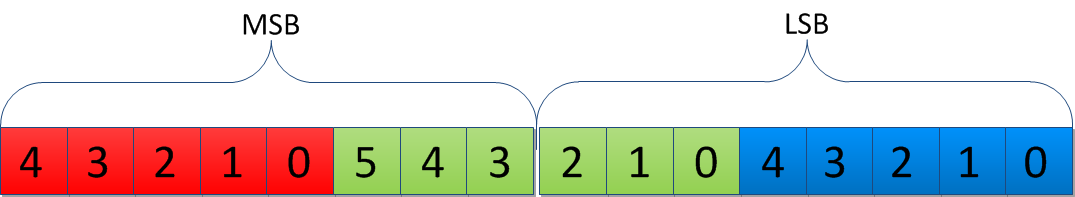
\includegraphics[width = \textwidth]{./Figures/RGB565.png}
\caption{RGB565 pixel format}
\label{fig:RGB565}
\end{figure}

The camera must use a high speed clock in order to ensure the pixels obtained are from the same time. This makes it difficult for an AVR to be able to respond to the camera quick enough (ATMegas typically clocked at 8-12MHz). This highlights the necessity for a FIFO Buffer. 

The OV7670 is set up so that the VSYNC pin goes low at the beginning of every full frame of data, and HREF is high when the data being output is valid. The pixel data is then clocked out on every rising edge of PCLK. To control the buffer, WEN (write enable) is NAND with the HREF signal. When both are high, the write enable to the buffer will be active and the data will be clocked in by PCLK. In order to acquire a full frame, the first VSYNC pin is set up to interrupt the AVR to enable WEN. The camera will output an entire frame of pixel data and store it into the buffer. When the second VSYNC is received, the WEN signal is disabled, stopping any more data being stored. The FIFO buffer now contains an entire image.

To obtain the data from the buffer, the AVR sets output enable and pulses the read clock. Valid data is available on the input port while RCLK is high. All the data is then read in half a pixel at a time. The entire operation can be seen in figure \ref{fig:ov_Capture}.
\begin{figure}
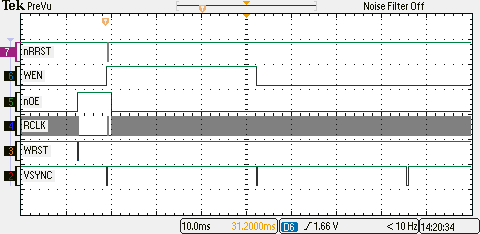
\includegraphics[width = \textwidth]{./Figures/ov7670_im_capture.png}
\caption{Signals generated to control the OV7670 capture and read}
\label{fig:ov_Capture}
\end{figure}


Difficulties arose at this point with the storage of the data. The ATMega644P has 4kB of internal SRAM, but  153.6kB of memory is needed to store a single image at QVGA (320 by 240 pixels, 2 bytes per pixel) quality. 

Firstly, data was sent straight to a desktop computer via a COM Port using USART. A simple desktop program was written in C\# to receive and store all the data, and to make a Bitmap image from the data. This method was slow, taking around 30 seconds to transmit one uncompressed image. 

The second option was to use extra memory connected to the microcontroller. An SD card is used as FAT file system so that data can be looked at by a user on a computer. Text log files are also written to aid debugging. This is discussed in section \ref{sect:SDCard}. 

\subsection{Dual Camera Operation}
In order for stereovision to be successful, two cameras separated by a horizontal distance ($B$) will need to be driven at the same time to obtain photos within a small time frame of one another.

A major problem occurred with using the \itc interface to set up both cameras. The camera has a set \itc address of $21_{16}$, which cannot be changed. Multiple \itc devices with exactly the same address cannot be used on the same bus. 
Two solutions to this are possible: driving one from $I^{2}C$ and one from SCCB, or using an \itc multiplexer. By using two different buses, there can be no bus contention. However, SCCB is slow and processor-hungry as it deals with the protocol bit by bit in software. This takes up memory and is not reusable for other operations.

An \itc multiplexer sits on the bus and has multiple output buses. The master can then address the multiplexer and select whether to pass the bus to bus 0, bus 1 or not allow the data to be transferred. This saves processor time, but means a write operation has to be done to select the camera bus before being able to write to the camera. This slows down the operation, but not as much as using SCCB. The main disadvantage to the \itc MUX is the extra hardware needed; firstly the MUX itself, but also 7 extra resistors to pull up the two extra buses and the three interrupt lines must be added. 

Overall, the disadvantages posed by using a MUX are small, so a multiplexer will be used as opposed to the SCCB interface. A suitable multiplexer is the Phillips PCA9542A \citep{I2C_Mux}.

The buffers have an output enable pin so the data bus can be shared by both cameras to the AVR. The ATMega644P offers three interrupt pins, two of which are used by the two VSYNC pins for the cameras.

Two ISRs are used to control the VSYNC signals, and when taking a photo, both frames are taken at a time period close together to capture the same scenario. The data for both images are read back individually by the AVR. 

Operation to read an image is identical to using one camera. However, an ID number is passed through the functions to make a decision on the pins to use to read the buffer and to enable the output. Care was taken to avoid bus contention, but no checking procedure is explicitly in place. Both images are then read back from the buffers and stored to memory. 

\section{SD Card} \label{sect:SDCard}

To use the SD card, the FATFS library \citep{FATFS} was used. The library supplies all the functions for writing a FAT File System in the files \textit{ff.c}, \textit{ff.h}, \textit{ffconf.h}, \textit{diskio.c}, \textit{diskio.h} and \textit{integer.h}. The \textit{diskio.h} functions control what device is being used - SD/MMC Card, USB drive etc. The \textit{ff.h} header contains all the functions to write to in a FAT File system. 
\\
An SD card was chosen due to it's small size, low cost and a large data storage. The cards work using an SPI bus which can be used for other devices within the system so the card only uses one extra enable pin in hardware to function. 

\subsection{Storing Images}

Many image formats are common, such as Joint Photographic Expert Group (JPEG), Portable Network Graphics (PNG), Bitmap (BMP) and Graphics Interchange Format (GIF). Table \ref{ImageFormats} shows a summary of some common image formats.


\begin{table}
\centering
\begin{tabular}{|p{3cm}| p{2cm}|p{2cm}|p{2cm}|p{2cm}|} \hline
			&	Bitmap 		& 	JPEG			 	&	PNG				& 	GIF \\ \hline
Extension 		& 	*.bmp 		&  	*.jpg /*.jpeg 		& 	*.png				& 	*.gif \\ \hline
Compression 	& 	No 			& 	Lossless  and Lossy		&	Lossless ZIP			&	Lossy	\\\hline
File Size of 320 by 
240 pixel Image (kB) &	225			&	20				&	23				&	24 \\\hline
Bits per Pixel		&	8, 16, 24 or 32	&	24				&	24, 32 or 48 			& 	24, but only 256 Colours \\


\hline
\end{tabular}
\caption{A table comparing different image formats available (\cite{ImageComparison})}
\label{ImageFormats}
\end{table}

It is clear that the best choice for images would be either PNG or JPEG. However, these require more computational time to compress the image into the correct format. To avoid compression, and thereby save processing time, bitmap was chosen at the expense of using more memory. The data in a bitmap image is also stored in RGB format so can be read back easily when processing the image. Appendix \ref{Chapter:AppendixB:BMPFile} shows the make up of a Bitmap File that was used.

By writing the image in this format, they are then able to be opened on any operating system. This aids debugging and allows the prototyping of image algorithms in a more powerful environment. Figure \ref{ExampleImage} shows a photo taken by the OV7670 and stored on a SD card.

\begin{figure}
\begin{center}
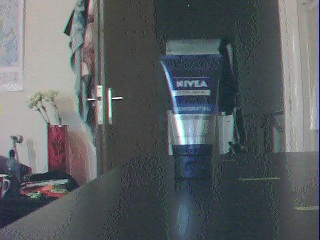
\includegraphics{Figures/ExampleImageFromCamera.jpg} 
\end{center}
\caption{An Example Image taken using the OV7670 and stored as a Bitmap on the SD Card}
\label{ExampleImage}
\end{figure}

\subsection{User Interface}
The ATMega 664P pinout for the dual camera operation can be seen in table \ref{table:644Pin}. Due to a lack of available GPIO pins, an ATMega168 was added on the \itc bus to act as a port extender. The ATMega168 accepts a read or write command. A write places the written data on Port D and a read returns any button pressed that occurred on Port C. When a button is pressed, this is stored in the ATMega168 until a read has been done. This is so the master (644P) does not miss any button presses while busy doing lengthy operations such as writing an image. The code is based on Application Note AVVR311 \citep{Atmel:I2CSlave}, written for IAR Compiler. This code was altered to compile with GCC under Atmel Studio. AVRs contain a hardware based \itc protocol that is interrupt based in software. The interrupt service routine of the TWI vector is a state machine which loads the data to send, stores received data, responds to acknowledges and address calls and deals with bus errors that can occur.

\begin{table}
\centering
\begin{tabular}{|c|c|c|c|c|}\hline
	& 	Port A 	& 	Port B 			& 	Port C 				& 	Port D 		\\ \hline
0	&	Data 0	&	SD Write Protect&	\itc - SCL			&	No Connection	\\
1	&	Data 1	&	SD Card Detect	&	\itc - SDA			&	No Connection	\\
2	&	Data 2	&	USB Data Plus	&	Read Clock 1		&	VSync 0			\\
3	&	Data 3	&	USB Data Minus	&	Read Reset 1		&	VSync 1			\\
4	&	Data 4	&	SPI Chip Select	&	Write Enable 1		&	Read Clock 0	\\
5	&	Data 5	&	SPI	MOSI 		&	Write Reset 1		&	Read Reset 0	\\
6	&	Data 6	&	SPI MISO		&	Output Enable 0		&	Write Enable 0	\\
7	&	Data 7	&	SPI Clock		&	Output Enable 1		&	Write Reset 0	\\
\hline

\end{tabular}
\caption{Pin Connections of the ATMega644P for Dual Camera Operation.}
\label{table:644Pin}
\end{table}
%\section{Motor Control}
%\inote{do something of this SOON}
\section{Circuit Development}
\subsection{Stereo Camera Development}
Figure \ref{sch:DualCam_Schematic} shows the circuit diagram for the prototype. This uses the Il Matto development board for the main microcontroller. The prototype can be seen in figure \ref{fig:Prototype}. This circuit captured and stored two images from the cameras to the SD card. 
\begin{figure}
\includegraphics[width=\textwidth]{./Figures/Prototype.jpg}
\caption{Prototype of Dual Camera operation.}
\label{fig:Prototype}
\end{figure}
\subsection{Motor Driver Development}
%\inote{Tachometers}
%\inote{Derivation of equations used - Distance / Rotating}
\inote{Testing of the Motor system - conclusion is likely to be that it is not a good method, need noise reduction}
\subsubsection{Hardware}
Tachometers are devices used to measure rotational speed of a shaft. Tachometers are most commonly found in bicycles where a small magnet is attached to the wheel and a sensor is attached to the frame. The sensor can then calculate the time period between rotations and therefore can calculate the speed (\citep{NEEDED}) \inote{Cite Needed}.

Here, an optosensor, TCRT1010, is used to measure rotations of the wheel and used to be able to move a distance decided by the microcontroller. The TCRT1010 package contains an IR LED and a phototransistor \citep{Vishay:TCRT1010:Datasheet}. The schematic of a simple transistor amplifier used can be seen in figure \ref{Circuit:TCRT1010} and was taken from \cite{NEEDED}. 
\inote{Cite Needed}
The wheel's rubber absorbed the IR, so a high voltage was always seen at the collector of the phototransistor. White tippex marks were applied to the wheels at regular intervals, which reflected IR and thereby giving a cheap way to detect wheel rotation. Figure \ref{Graph:WheelVoltage} shows the voltage at the collector (read by the ADC on the AVR) against the angle of the wheel. Five white tabs were marked on the wheel, and five dips in the voltage can be seen in figure \ref{Graph:WheelVoltage}. 

\inote{Maybe do some simulations of this circuit? This could dictate a maximum speed}

\begin{figure}
\centering
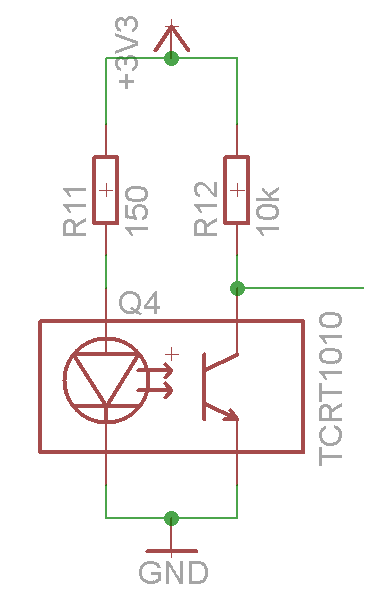
\includegraphics[scale=0.5]{Figures/TCRT_Circuit.png}
\caption{Circuit diagram of Optosensor}
\label{Circuit:TCRT1010}
\end{figure}

\begin{figure}
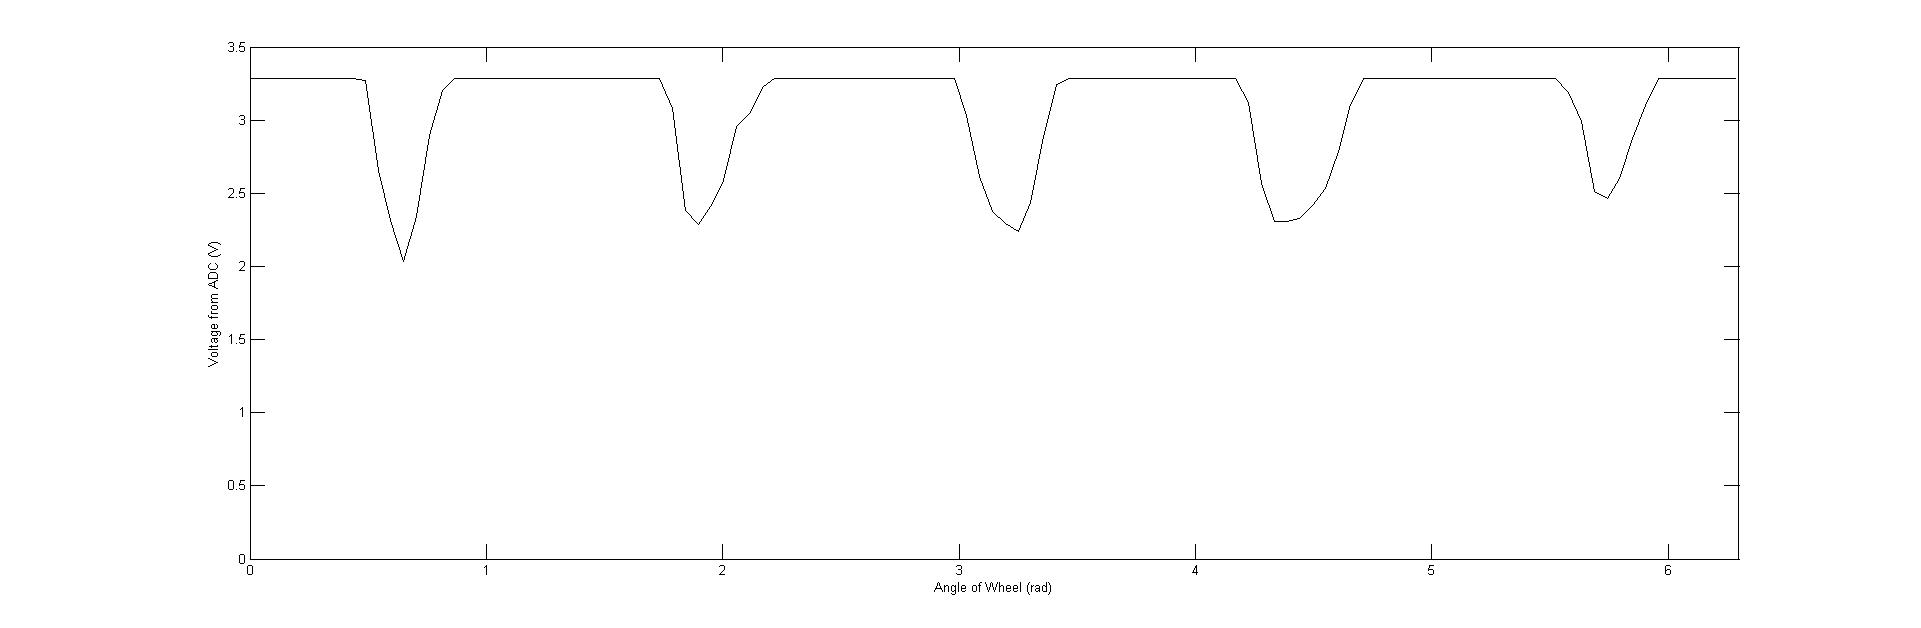
\includegraphics[width = \textwidth]{Figures/WheelVoltageGraph.jpg}
\caption{Graph of Wheel Angle against the Voltage read by the AVR}
\label{Graph:WheelVoltage}
\end{figure}

%\subsubsection{Derivations of Movement Calculations}
%Two basic movements were decided to be implemented: Straight line and rotation. 

\subsubsection{Firmware Development}

As the voltage swing from the phototransistor does not reach 0V, the AVR cannot detect this as a logical 0. The internal ADC can be used to continually read the analogue voltage from the phototransistor and detect low points from this data. This method requires the processor to continually compare values and process the data. However, more control would be had over the noise in the data.

An alternative is to use an analogue comparator built in on most AVRs. This can be set up to run an interrupt service routine when the voltage crosses a threshold. The threshold voltage can be determined by a potentiometer. The code is primarily two methods, the set up and the ISR.

Set up is different for if a rotation or movement is wanted. Moving in a straight line takes a parameter of how far to move as a signed integer and calculates the total number of interrupts that need to occur can be calculated using \eqref{eq:NumberInterrupts}. This value is put in a global variable. The PWM and input pins to set the correct direction are then set up before enabling the motor. 

\begin{equation}
\label{eq:NumberInterrupts}
Interrupts = D \times \frac{IPR}{C_w}
\end{equation}

To rotate, one of three methods can be used: Spot rotation on the centre of the robot, or pivot on either left or right wheel. For ease, the Spot rotation is the only one implemented. To calculate the distance moved, the radius to the wheels needs to be known. The circumference through the wheels is then easily calculated and the angle of rotation is then a ratio. The distance to move is calculated by equation \eqref{eq:RotationalDistance} and the total number of interrupts can be calculated using equation \eqref{eq:NumberInterrupts}. To rotate clockwise, the left motor is driven forward and the right is driven backwards. To rotate anti-clockwise, the directions are reversed

\begin{equation}
\label{eq:RotationalDistance}
D_{R} = A \times \frac{C_b}{360}
\end{equation}

Combining equations \eqref{eq:NumberInterrupts} and \eqref{eq:RotationalDistance} gives:
\begin{equation}
\label{eq:RotationalInterrupts}
Interrupts = A \times \frac{IPR}{C_w} \times \frac{C_b}{360}
\end{equation}
Where $A$ is the angle to rotate in degrees, $IPR$ is the number of interrupts generated per full revolution of the wheel, $C_w$ is the circumference of the wheel and $C_b$ the $2\pi\times r_b$ and $r_b$ is the distance from the centre of the robot to the centre of the wheel (see figure \ref{fig:RobotBase_Annotated}).



\begin{figure}
\centering
\subfigure[Top View of robot base showing dimensions of interest\label{fg:RobotBase:Top}]{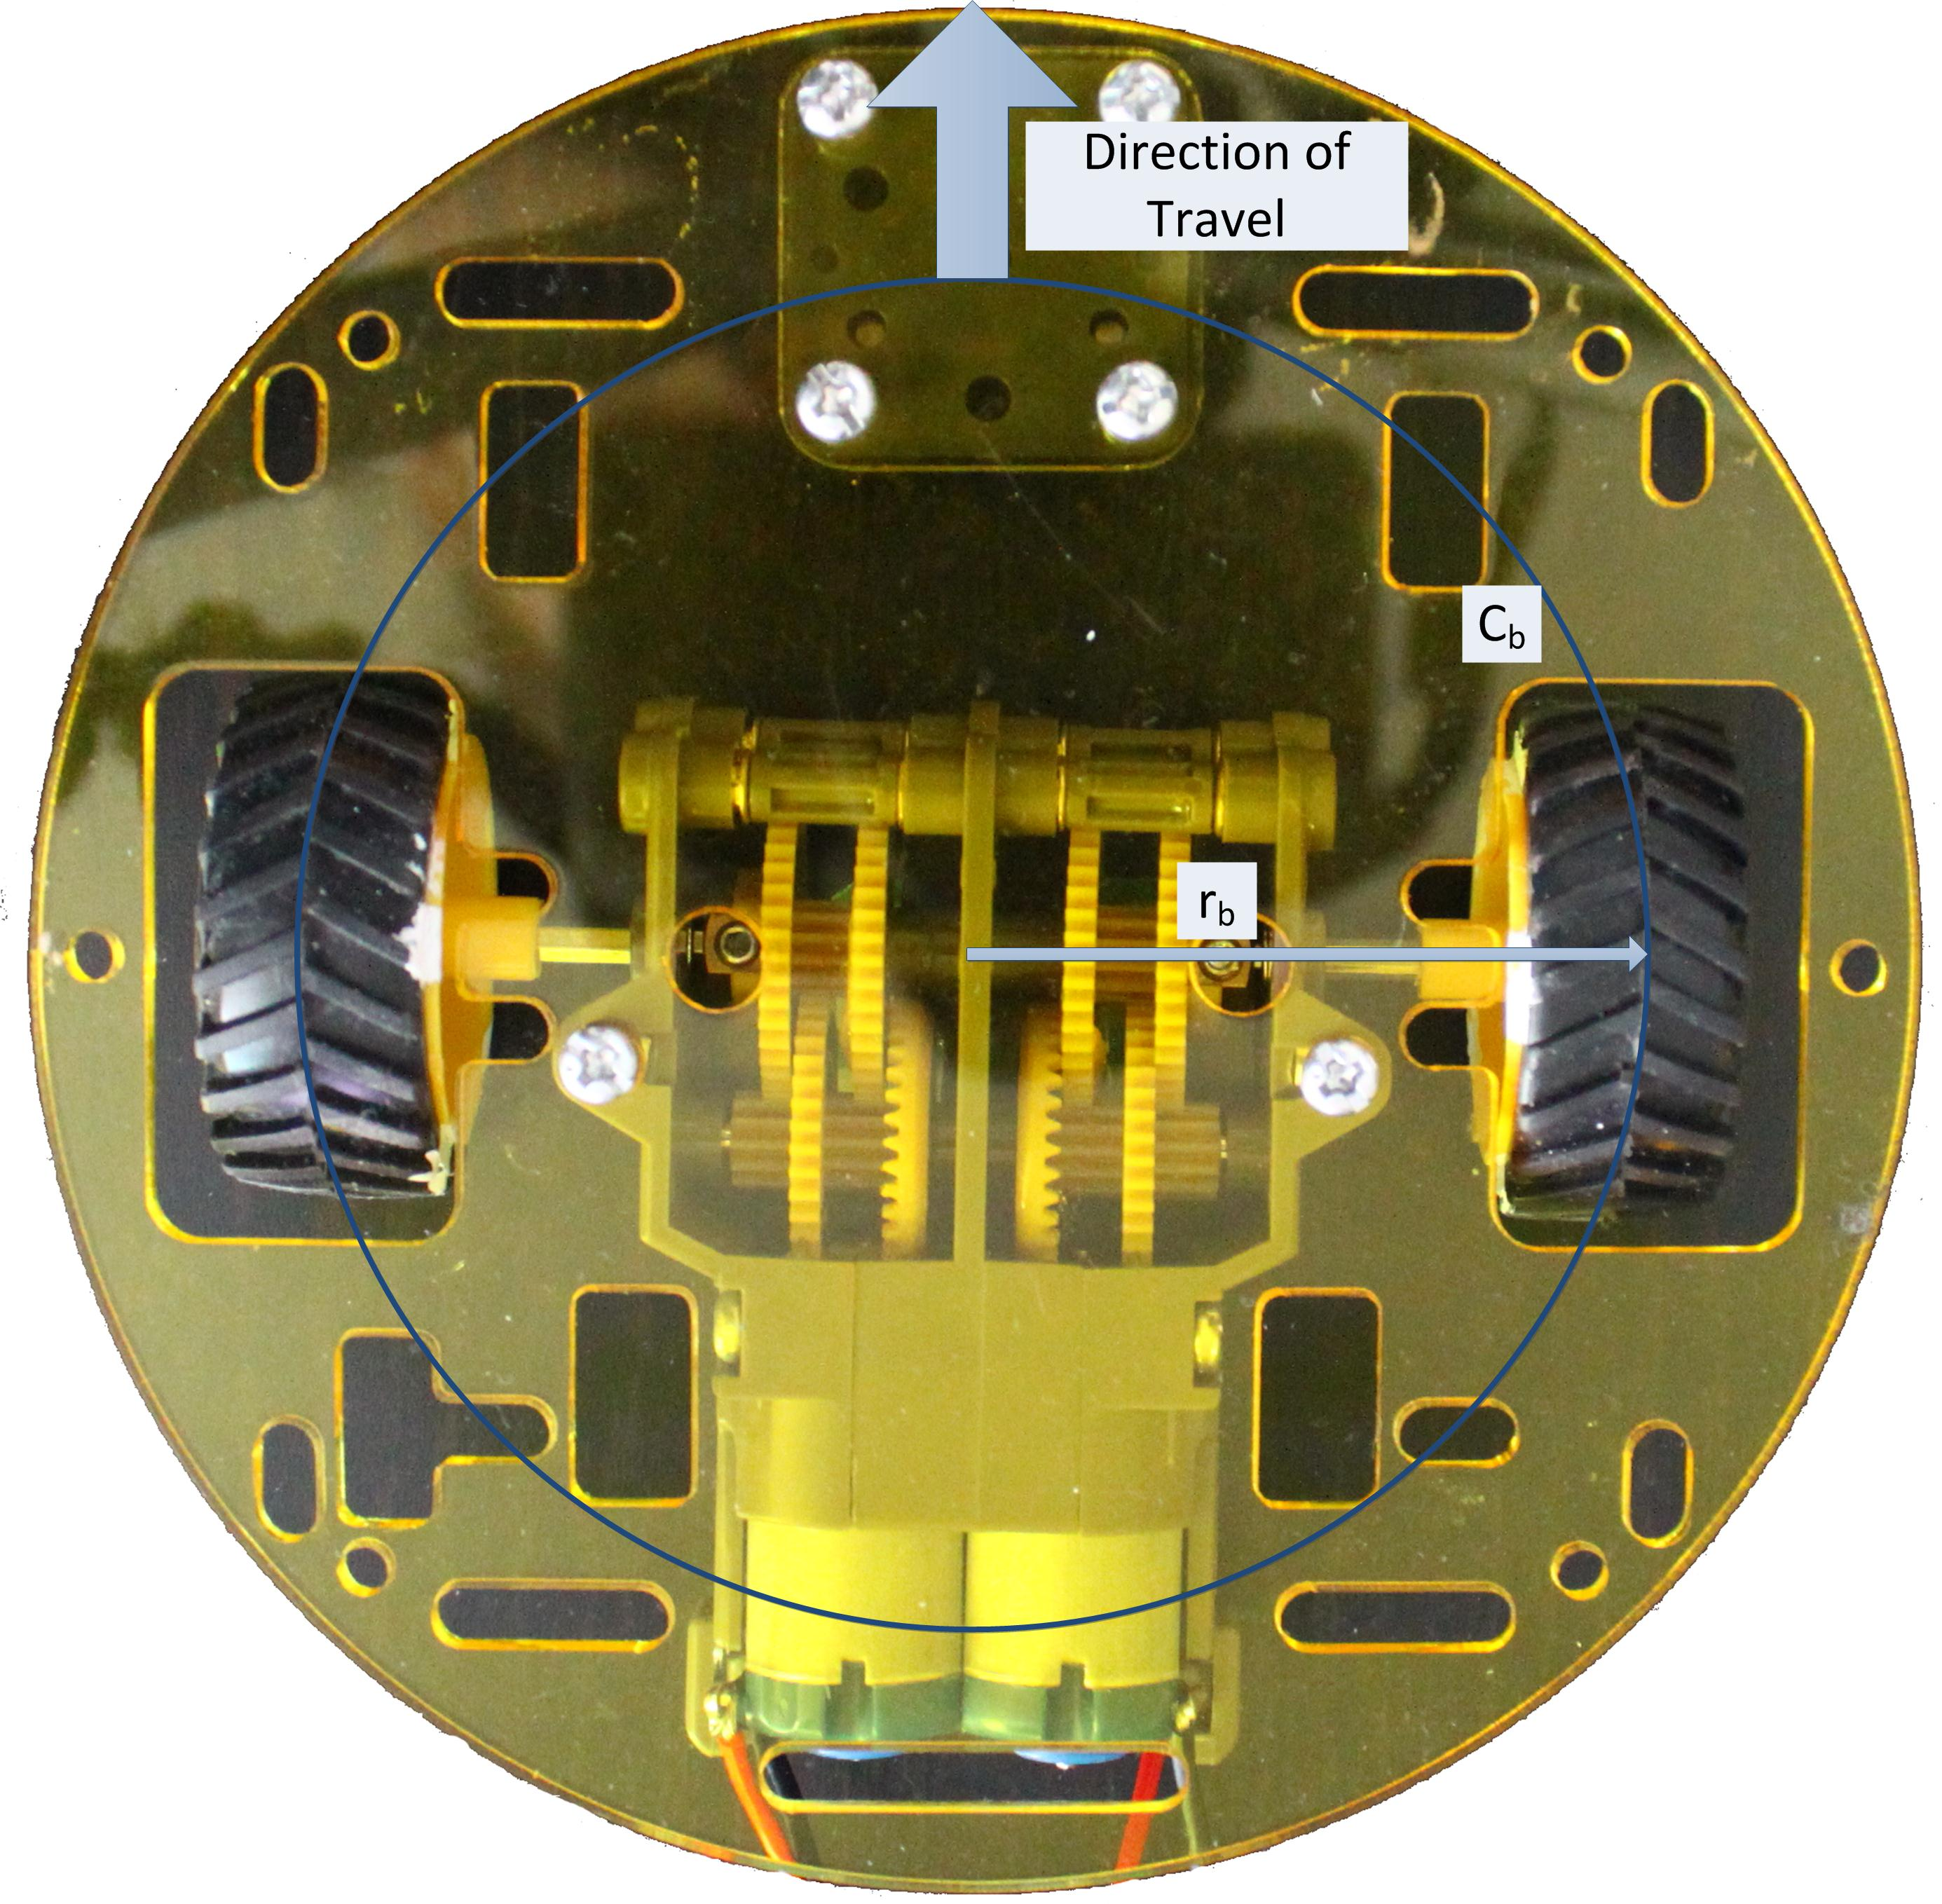
\includegraphics[width = \textwidth, keepaspectratio]{./Figures/Robotbase_top_annot.jpg} }
\subfigure[Side View of robot base showing dimensions of interest\label{fg:RobotBase:Side}]{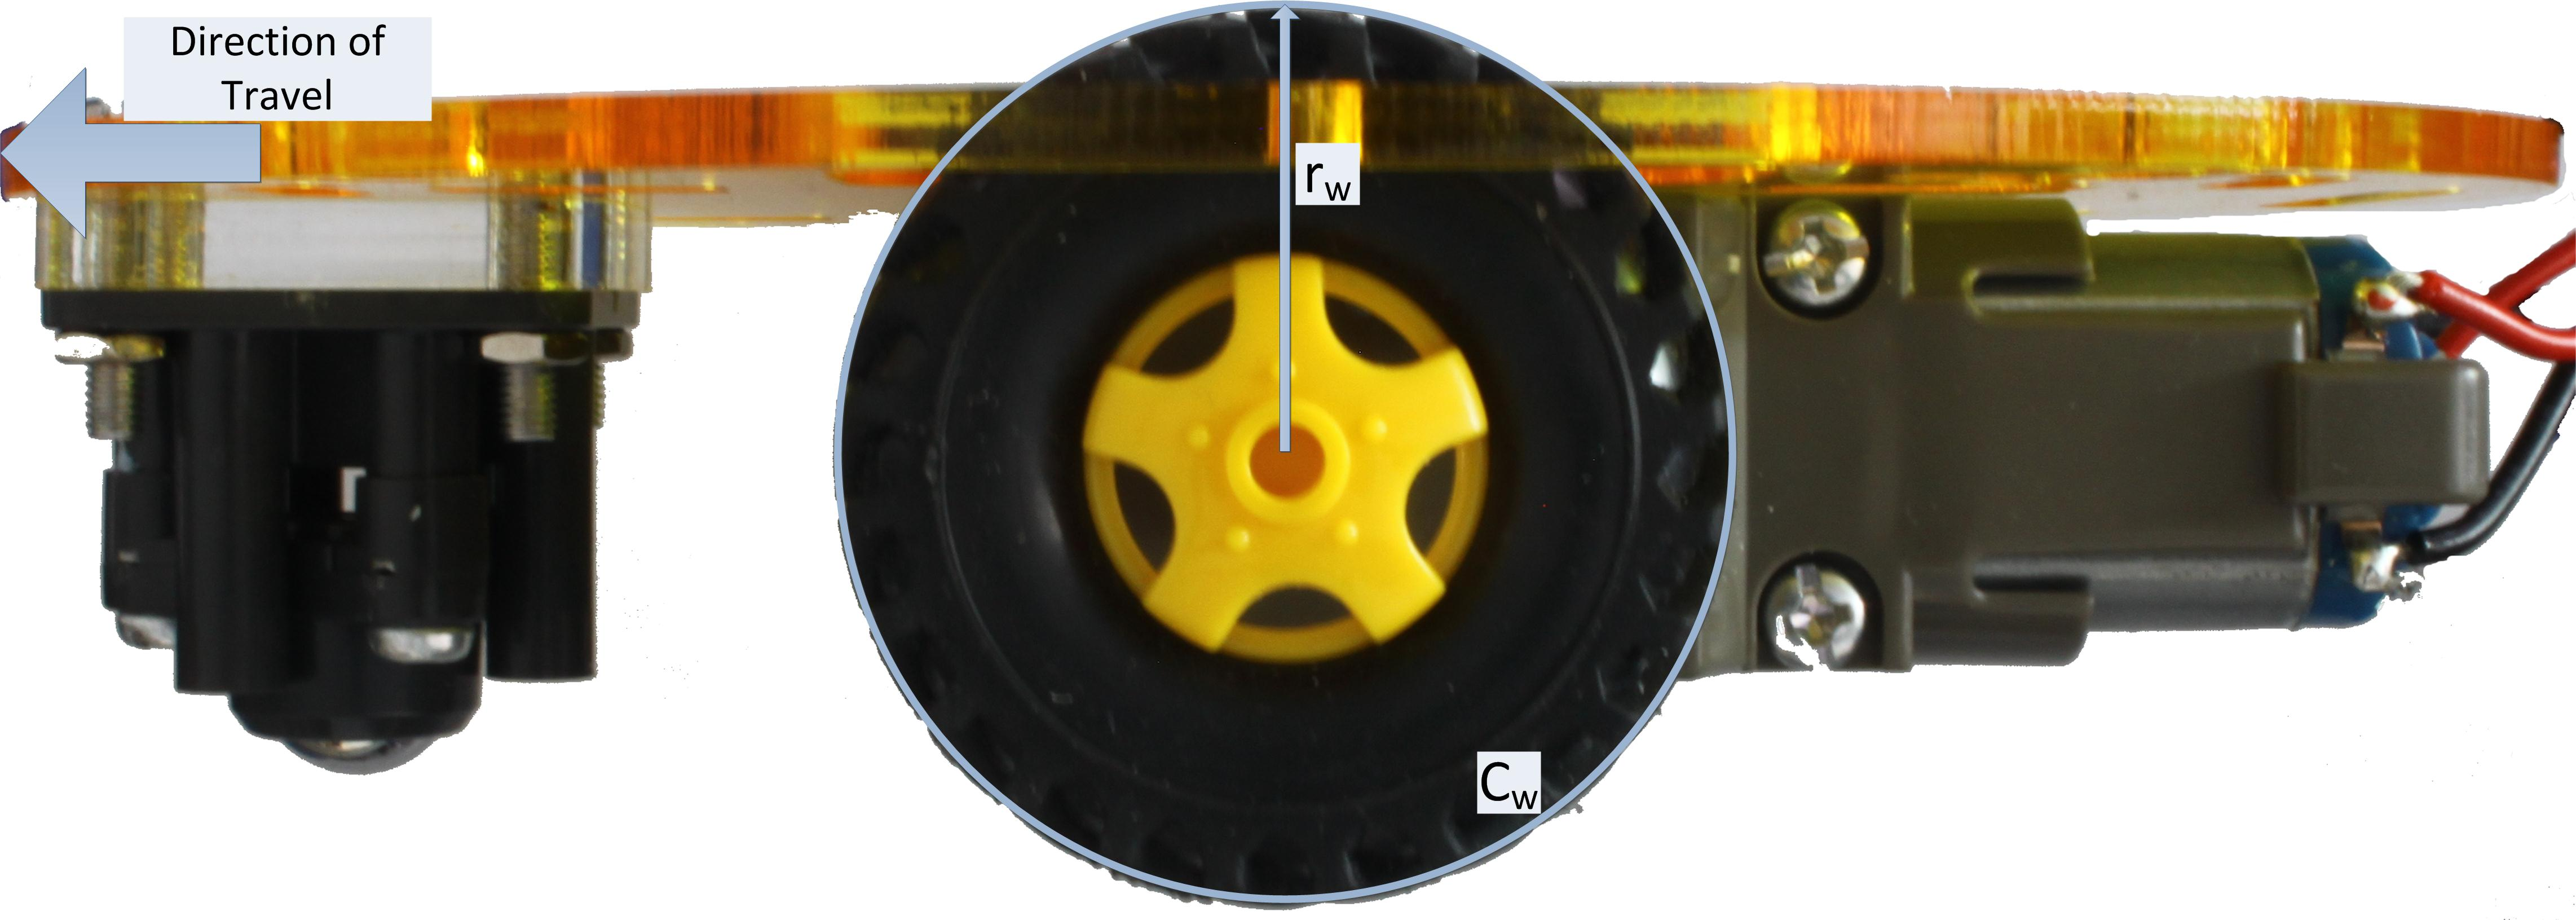
\includegraphics[width = \textwidth, keepaspectratio]{./Figures/Robotbase_side_annot.jpg} }
\caption{Dimensions of Interest for Robot Movement}
\label{fig:RobotBase_Annotated}
\end{figure}
\inote{Maybe a figure to explain better?}


The motor speed can be controlled by Pulse Width Modulation (PWM). The code sets up a low duty cycle PWM signal to drive the motors slowly. This removes the need for a controller to ensure the correct distance was moved. 

The final code can be seen in appendix \ref{Chapter:AppendixC:Code}
\subsubsection{Testing}\label{Section:MotorTest}
\inote{Need to get the motors to work reasonably first}
\subsubsection{Conclusion}
\inote{It doesn't work}

\section{PCB Development}
\subsection{Circuit Design}
The circuit diagram for Revision A can be seen in section \ref{sch:Columbus:CircuitDiagram}. The schematic for the SDRAM and values and locations of decoupling capacitors were taken from the schematic of the UC3C-EK development board \citep{Atmel:UC3CEK}. 
\subsection{PCB Design}
The PCB was designed using EAGLE CAD Software. A four layer board was decided to be used to save space when routing Power. Layer 2 is a 3V3 plane and layer 3 is a ground plane. A ground plane is also on the top and bottom layers to help eliminate any ground bounce that could occur. 

The SDRAM uses the EBI protocol. In high speed systems, care is often taken to equalise track lengths \citep{liu2004equalization}. The UC3C maximum clock frequency is 33MHz (with no wait states), which is not fast enough to cause any track equalisation problems. Care, however, was taken on the USB lines to ensure correct impedance and the tracks lengths matched to each other.

Tracks were routed in order of priority, starting with the UC3C, SDRAM and cameras, and then other devices were routed, \itc MUX, SD card, motor drivers etc. As a precaution, spare pins from the UC3C were routed to a header (J8 and J9) so that additions could be done if a pinout or connection was found to be incorrect. Also, UART, \itc and SPI connections were routed to headers J7, J4 and J5 respectively so logic analysers and COM Port could be attached easily for debugging.

Most of the passives used were 0603 size, but some 1206 capactitors were used for decoupling the voltage regulator and a 1206 diode was used for the analogue reference circuitry. LEDs were also 1206 size. All headers were 0.1'' spaced and a mini B USB socket was used. 

The layout of components was important. The cameras needed to be as far apart as possible and at the front of the PCB. The motor drivers were situated toward the back of the PCB and 0.1'' headers were added to connect the motors to. The optosensors were positioned such that they could be mounted directly on the PCB and be in the correct position to sense the wheels. Mounting holes were also added onto the board so the PCB could be mounted on to the robot base easily. The overall dimensions of the PCB were $100mm \times 70mm$. A full list of components and cost of each is documented in table \ref{table:Costings}


\begin{table}
\centering
\begin{tabular}{|c|p{2cm}|c|c|c|} \hline
Component	&	Cost per unit (\pounds)	& Quantity 	&	Cost (\pounds)	&	Source		\\ \hline
Capactiors	&	0.155 					& 	43		& 	6.67 					& 	Farnell 	\\
Clock 		& 	1.48					& 	1		&	1.48 					& 	Farnell		\\
Diode		&	0.48					&	1		&	0.48					&	Farnell 	\\
Headers		&	0.51 					&	5		&	2.55					&	Farnell 	\\
I2C Mux PCA9542A &	0.81				&	1		&	0.81					&	Farnell		\\
LEDs 		&	0.158					&	7		& 	1.11 					&	Farnell		\\
Micro SD Card &	4						&	1		&	4.00 					&	Amazon 		\\
Micro SD Card Connector & 2.04			&	1		&	2.04					&	Farnell		\\
AT32UC3C0512C	&15.39					&	1		&	15.39					&	Farnell		\\
TB6593FNG 	&	1.07 					&	2 		&	2.14 					&	Farnell 	\\
Motors  	&	0.42					&	2		&	0.84				 	&	Rapid 		\\
TCRT1010	& 	0.94 					&	2		&	1.88 					&	Farnell 	\\
OV7670		&	17						&	2		&	34.00					& 				\\
Potentiometer	&	0.43				&	2		&	0.86					&	Farnell 	\\
Resistors	&	0.066 					& 	46		&	3.04 					&	Farnell 	\\
MT48LC4M16A2P	& 3.24  				& 	1		&	3.24 					&	Farnell		\\
Switch		&	0.45					&	1		&	0.45					&	Farnell 	\\
USB Socket	&	0.84 					&	1		& 	0.84 					&	Farnell 	\\
LM1117MP	&	1.03					&	1		&	1.03	 				&	Farnell		\\ \hline \cline{3-4}
\multicolumn{2}{c|}{ }					& Total Cost  & \pounds 82.84			&	\multicolumn{1}{|c}{ }			\\ \cline{3-4}
\end{tabular}
\caption{A table of all components used and their costs.}
\label{table:Costings}
\end{table}

Finally, the name ``The Columbus'' was decided on as the original application for the project was a mapping robot that would search out an unknown area, so the robot was named after Christopher Columbus who explored and navigated parts of the American continents which were unknown at the time. The Eagle CAD Diagram of the PCB can be seen in Appendix \ref{Appendix:PCB}. The PCB was manufactured by \cite{PCBCart}. The PCB cost \pounds 205 to manufacture and ship. A photo of the PCB can be seen in figure \ref{fig:PCB:Bare}. 

\begin{figure}
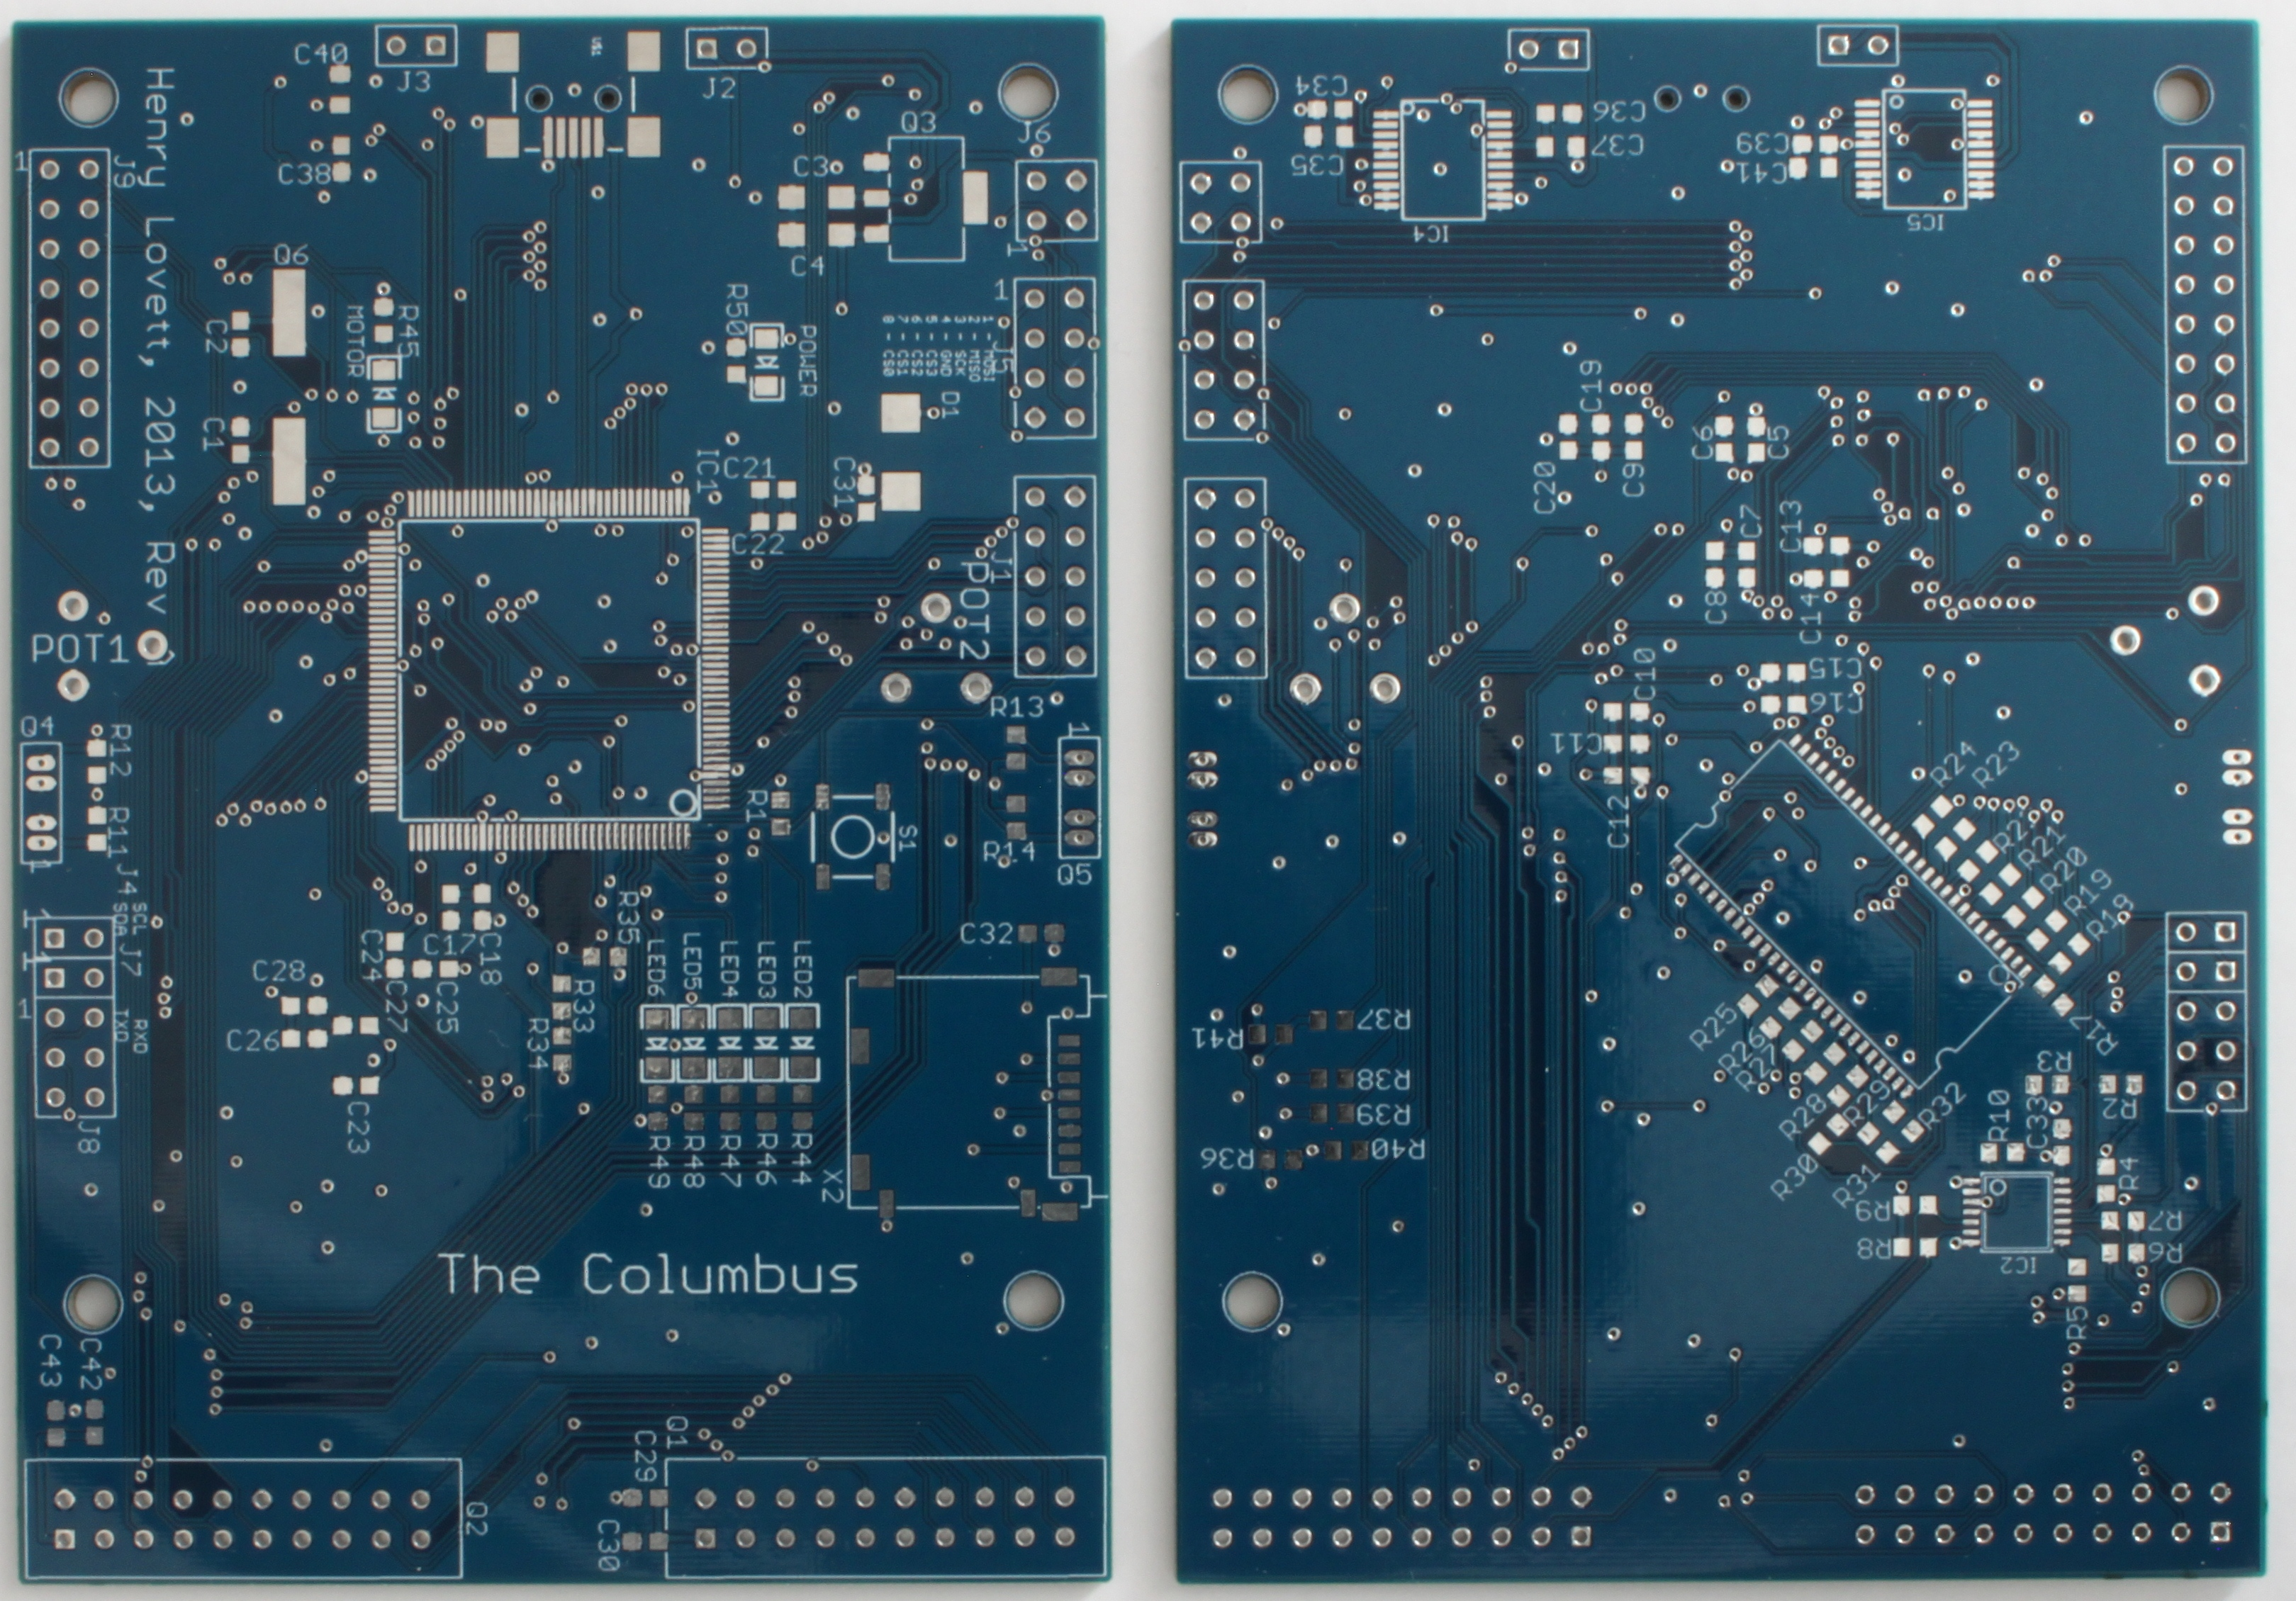
\includegraphics[width=\textwidth]{./Figures/PCB_Bare.jpg}
\caption{PCB with no components. Left: Top View. Right: Bottom View}
\label{fig:PCB:Bare}
\end{figure}

\inote{Considerations - Power consumption of devices not exceeding VReg}

\subsection{PCB Testing}
A program was written to test all the devices on the PCB. The following tests are done:
\begin{enumerate}
\item UART Send and Receive
\item SD Card Test
\item All LEDs on and off
\item SDRAM Test
\item \itc Test
\item Camera Test
\item Motor Test
\end{enumerate}
The folowing sections explain the tests done to check the devices and protocols worked.

\subsubsection{UART Test}
When the test program begins, the microcontroller waits for a character input. All characters are echoed back. This enables the user to check the communications work. Once a carriage return key is received ($13_{10}$), the test program continues. Listing \ref{lst:UARTTestCode} shows the test code for the UART protocol.

\lstinputlisting[style=C,caption=UART Test Code,label={lst:UARTTestCode},frame=single,numbers=left,tabsize=2,breaklines=true, firstline=110,lastline=121]{../Code/ColumbusTest/ColumbusTest/src/main.c}


\subsubsection{SD Card Test}
The Atmel Software Framework \citep{Atmel:ASF} provided drivers and code for SPI communications and use of a FAT32 File System. The code was configured to use the correct Chip Select pin for the SD Card and the correct SPI Bus was also configured. The test consists of initialising the memory, reading the capacity of the card and printing it to the user. 

The AVR then proceeds to delete any previous log file, create a new log file and writes \textit{``Columbus Tester''} to it. The first 8 characters, which should be \textit{``Columbus''} are read back and checked.
\lstinputlisting[style=C,caption=UART Test Code,label={lst:SDTestCode},frame=single,numbers=left,tabsize=2,breaklines=true, firstline=124,lastline=196]{../Code/ColumbusTest/ColumbusTest/src/main.c}

This exercises all basic File I/O functions, creating, reading and writing and checks them on the device.

\subsubsection{LED Test}
All LEDs are turned on for 1 second, and then turned off. The user should check this occurs. It verifies that all the LEDs are functional and correctly mounted. The Power LED should be on when power is supplied to the PCB. 

\subsubsection{SDRAM Test}
The SDRAM test consists of initialising the SDRAM, calculating the SDRAM Size, writing a unique test pattern to the whole memory, and then reading it back and checking it. The total number of errors are reported. 

The test was adapted from an Example Application from the Atmel Software Framework \citep{Atmel:ASF}. The code can be seen in listing \ref{lst:SDRAMTestCode}. It consists of two \textit{for} loops. In the first, the iteration number is assigned to the memory location. The second loop reads back the data and checks it is correct. An int, \textit{noErrors}, is used to count errors. 

\lstinputlisting[style=C,caption=SDRAM Test Code,label={lst:SDRAMTestCode},frame=single,numbers=left,tabsize=2,breaklines=true, firstline=217,lastline=258]{../Code/ColumbusTest/ColumbusTest/src/main.c}

\subsubsection{\itc Test}
The \itc test checks the bus for devices. It prints out a table showing the address of any devices that acknowledge a probe. A probe is a set up to write to the address. If a device exists on the line, it should Acknowledge \citep{Philips:I2C}. The test is done three times, with no channel selected on the \itc MUX, with channel 0 selected and with channel 1 selected. The two addresses expected at $21_{16}$ for the OV7670 Camera and $74_{16}$ for the \itc MUX. The camera should only acknowledge when the \itc MUX has the relevant channel selected. Listing \ref{lst:TWITestCode} shows the test code for the \itc bus and listing \ref{lst:TWITestCode} shows the result from the full bus scan with channel 0 selected. The cameras are both checked to exist.
\lstinputlisting[style=C,caption=\itc Test Code,label={lst:TWITestCode},frame=single,numbers=left,tabsize=2,breaklines=true, firstline=268,lastline=315]{../Code/ColumbusTest/ColumbusTest/src/main.c}

\begin{lstlisting}[caption={Result of \itc bus scan with Channel 0 of the \itc MUX selected},label={lst:I2CTest}]
Scanning Channel 0
h 0 1 2 3 4 5 6 7 8 9 A B C D E F
0 - - - - - - - - - - - - - - - -
1 - - - - - - - - - - - - - - - -
2 - A - - - - - - - - - - - - - -
3 - - - - - - - - - - - - - - - -
4 - - - - - - - - - - - - - - - -
5 - - - - - - - - - - - - - - - -
6 - - - - - - - - - - - - - - - -
7 - - - - A - - - - - - - - - - -
\end{lstlisting}

\subsubsection{Camera Test}

This test consists of initialising both cameras and checking it passes. Two photos are then taken and stored to the SD card. Success or Failure is displayed. Two images should exists on the SD card from the two cameras. Listing \ref{lst:CameraTestCode} shows the code to conduct this test.
\lstinputlisting[style=C,caption=Camera Test Code,label={lst:CameraTestCode},frame=single,numbers=left,tabsize=2,breaklines=true, firstline=316,lastline=338]{../Code/ColumbusTest/ColumbusTest/src/main.c}

\subsubsection{Motor Driver Test}
An extensive test of the motor driver is discussed in section \ref{Section:MotorTest}. The test code in this application resets the motors so that they are aligned to a white tab on the wheel. This code can be seen in listing \ref{lst:MotorTestCode}. The robot should move no further than 2cm to reach a white tab and the motors should drive forward. This test is useful here to ensure the motors are connected the correct way around and that the potentiometers are set to an appropriate level.

\lstinputlisting[style=C,caption=Motor Test Code,label={lst:MotorTestCode},frame=single,numbers=left,tabsize=2,breaklines=true, firstline=339,lastline=346]{../Code/ColumbusTest/ColumbusTest/src/main.c}

\subsection{PCB Faults}
During the build and test of the PCB, a number of faults were found. Each is explained and the solution for the problem given. 
\subsubsection{SDRAM Footprint}
The SDRAM footprint made was done exactly to the specification of the pad size and locations with no consideration for soldering to. This meant the chip fit exactly on to the footprint. This made soldering difficult as pads had to be preloaded with solder and the device's pins were heated and bound to the solder. The chip does not seat flat against the PCB. It also put the device at risk as more heat had to be used that usually necessary. Figure \ref{fig:SDRAM_Err} shows the SDRAM chip against the footprint. There is no extra space on the pad to be able to easily solder the device.

\begin{figure}
\centering
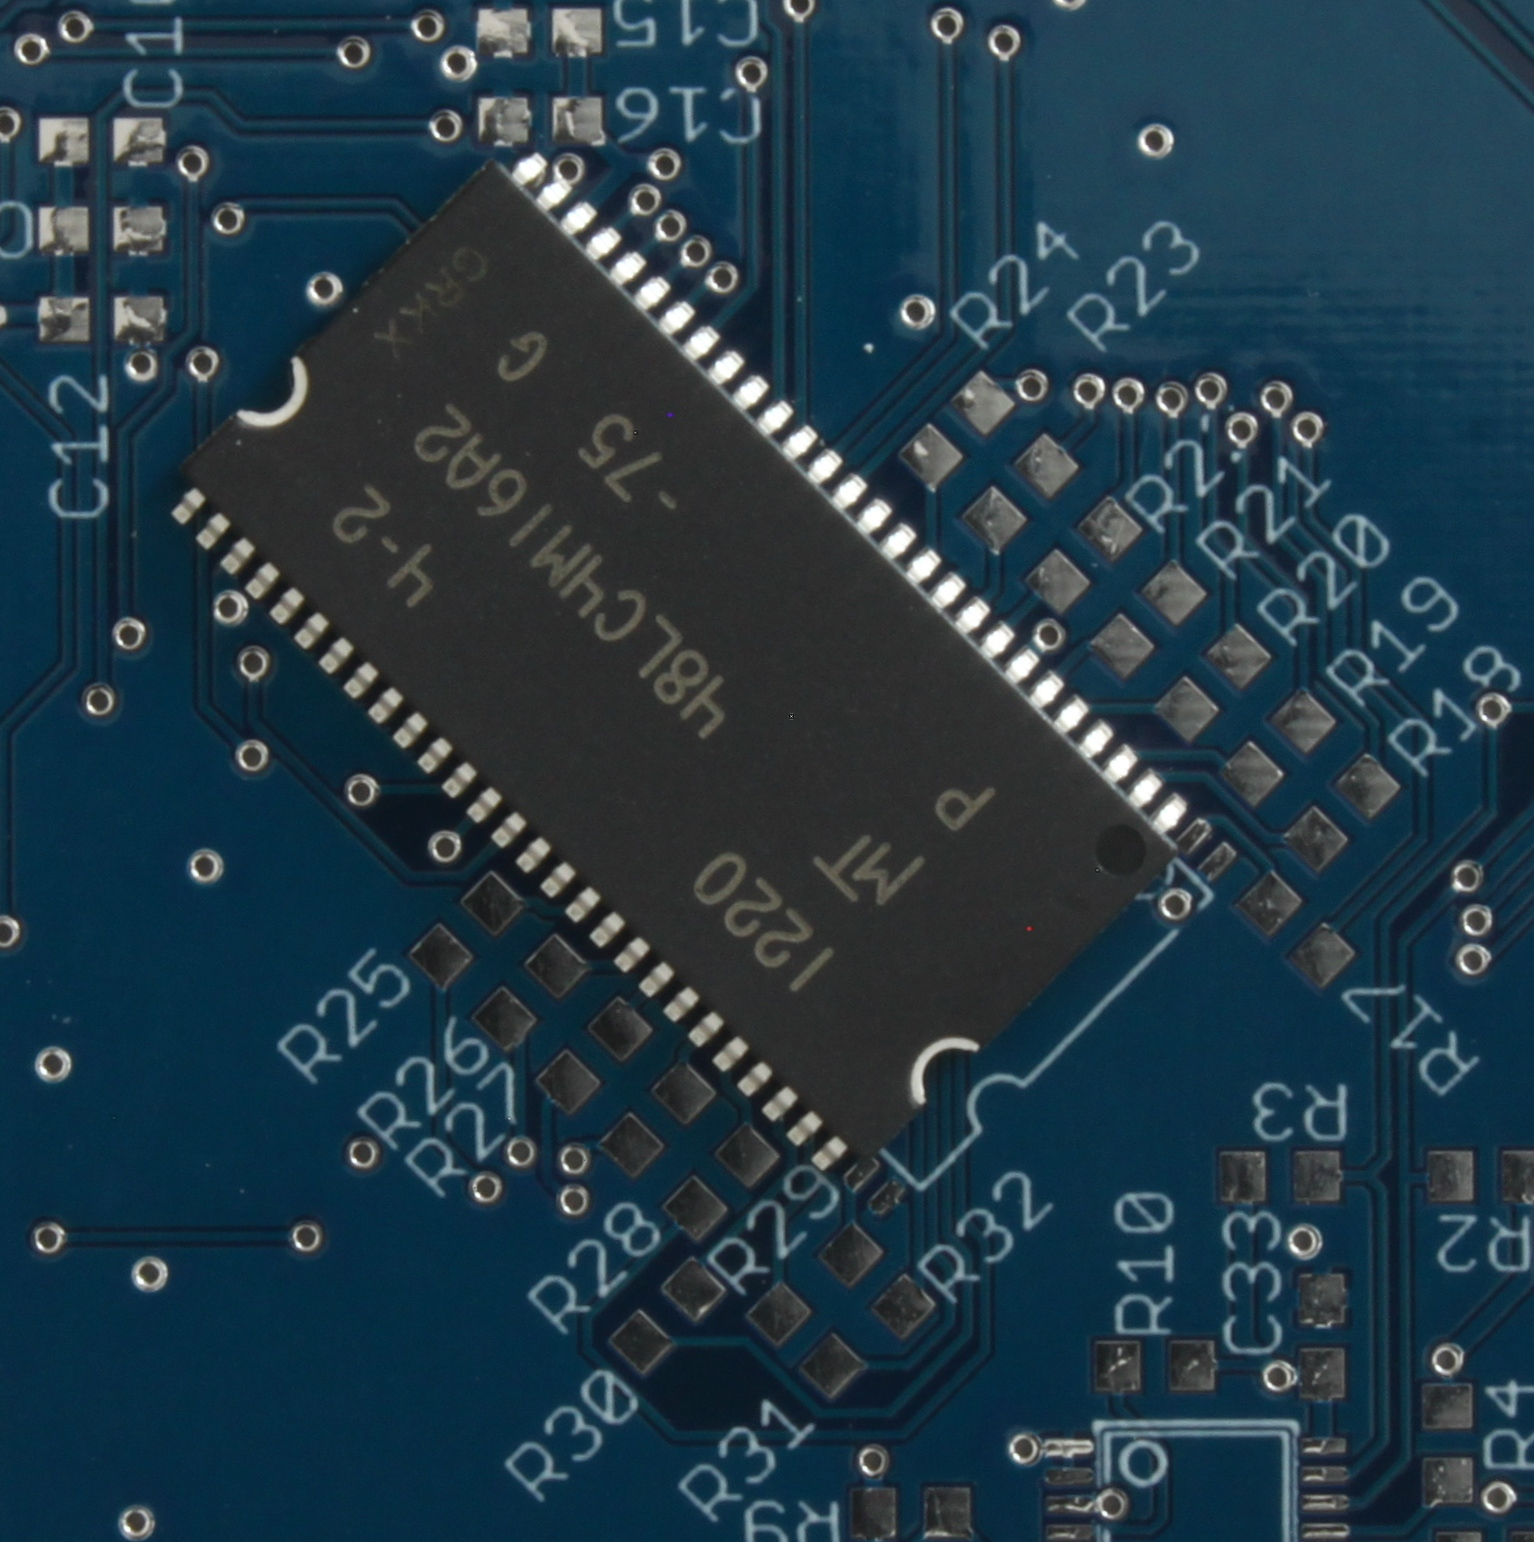
\includegraphics[width=\textwidth / 2]{./Figures/PCB_SDRAM.jpg}
\caption{SDRAM Chip shown against its footprint.}
\label{fig:SDRAM_Err}
\end{figure}

To avoid this, existing footprints could be used from other libraries, or double checking the footprints made. The problem meant extra care during soldering had to be taken but has not impeded the operation of the device. 

\subsubsection{SDRAM Chip Select}
The code was prototyped on the Atmel UC3C-EK development board prior to the PCB arriving. When the PCB was built, the code did not work, even with the Chip Select declaration changed. To diagnose this problem, the control lines of the SDRAM were probed with a logic analyser. On the UC3C-EK, the bus was busy with refresh cycles outside of SDRAM access. On the Columbus, no activity was seen. 

The reason the correct control wasn't being seen was due to the UC3C device having a dedicated SDRAM controller, attached to only Chip Select line 1. The Columbus was designed to used chip select line 0. Chip select 1 was available on an external pin, and a via through the routing was close to a via connected to the SDRAM chip select line. Therefore, to overcome the problem, a small enameled wire was soldered to join the two vias together. This solved the problem and the correct signals were then seen on the control lines. The patch can be seen in figure \ref{fig:PCB:Bottom}. 

This fault was caused by not reading the datasheet carefully and ignoring a proven circuit diagram. 

\subsubsection{SDRAM Data Line Resistors}
Once the chip select problem was solved, data returned was unreliable. The SDRAM is word (32 bit) addressed, but accessed in 16 bits. This means read cycles are done per word read. 
Upon investigation of this problem, the 14th, 15th, 30th and 31st (top two bits of each 16 bit access) seemed to read as a 1 the majority of the time. This result wasn't repeatable and sometimes returned correct data. The other bits of the data were always correct. Table \ref{table:SDRAM_Err} shows some examples of the problematic data bits. The data written should match the data read back. 

\begin{table}[!ht]
\caption{A table showing examples of the incorrect data returned from the SDRAM}
\label{table:SDRAM_Err}
\begin{tabular}{c c}
Data Written							&	Data Read \\
00000000 00000000 00000000 00000000		&	\textcolor{red}{11}000000 00000000 \textcolor{red}{11}000000 00000000 \\
00001111 00001111 00001111 00001111		&	\textcolor{red}{11}001111 00001111 \textcolor{red}{11}001111 00001111 \\
\end{tabular}
\end{table}

The problem was traced to resistors \textbf{R31} and \textbf{R32}. They were soldered on incorrectly so that the two data lines of the SDRAM were connected together and the two AVR GPIO pins were connected together. Data was then read back from, effectively, a high impedance line and therefore varied. Once the resistors were soldered correctly, the issue no longer persisted and the whole SDRAM test passed. By utilising the soldermask more, device orientations could be added to ensure correct placement. This can be extended to other devices, such as diodes and capacitors, especially in densely populated areas. 

\subsubsection{Camera Interrupt Line}

As discussed in section \ref{Section:Camera}, the OV7670 needs an interrupt line to synchronise quickly to the start of the frame and is done by using an interrupt line. The UC3C0512C has 9 external interrupt lines. On the PCB, interrupt lines 0 and 1 were used for this control.

Interrupt line 1 was easily configured and worked as expected. However, interrupt 0 did not seem to trigger the interrupt service routine. It was found that interrupt 0 was a ``Non Maskable Interrupt'' which has specific uses and cannot be used in to trigger a method. 

The external interrupt 4 pin was wired to Junction 8 on the PCB. A wire was attached to the camera's VSYNC line and attached to the relevant pin on the header. The operation was then easily obtained and the VSYNC line triggered correctly.

This issues would have been avoided with more understanding of the device before hand and checking the datasheet.


\subsubsection{Motor Driver Pinout}

An error was made in creating the device for the TB6593FNG Motor Driver in EAGLE. On the device, each motor output has two pins to drive each side of the motor. The pin assignment was mixed up when created and connected the two outputs together. Figure \ref{fig:Motor:Error} shows the track errors on one of the motor drivers. 

\begin{figure}
\centering
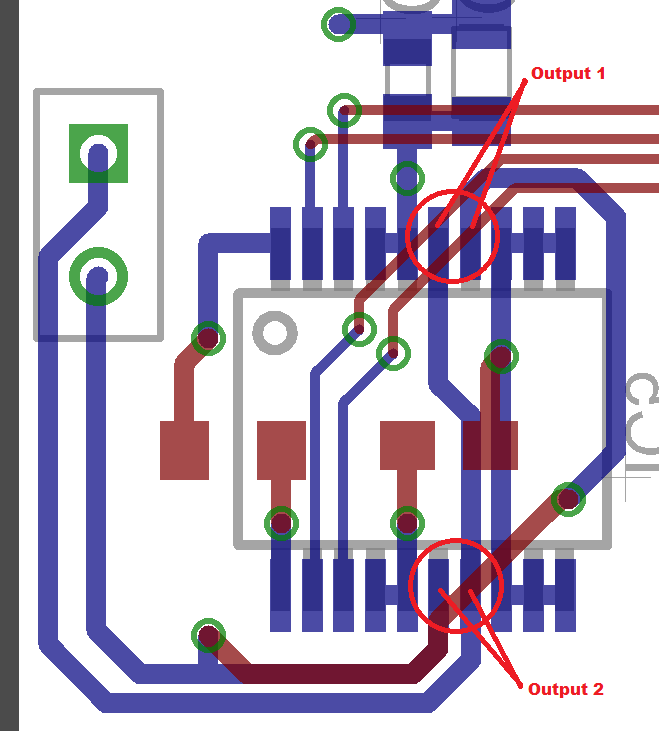
\includegraphics[width = \textwidth /2]{./Figures/MotorDriver_error.png}
\caption{Motor Driver error. Outputs incorrectly connected}
\label{fig:Motor:Error}
\end{figure}

To solve this, pins 7 and 14 were lifted and removed so that output 1 and output 2 were not connected together. The devices were not damaged in the process of testing this and the motors functioned correctly after this. Double checking the footprints made against the datasheet would have avoided this problem. No impedance to the operation of the drivers has been seen, but the patch may hinder the devices ability to sink current to the motors. 

\subsection{PCB Conclusions}
A number of faults were made in the PCB design. They are:
\begin{itemize}
\item SDRAM footprint
\item SDRAM chip select line
\item SDRAM data line resistors
\item Camera interrupt line
\item Motor driver pinout
\end{itemize}
Three of the faults could have been avoided by consulting the datasheet more carefully during the circuit design stage. The footprint error was due to not being experienced in designing footprints and the data line resistors was a mistake due to lack of attention being paid. 

For future PCBs, more care will be taken in circuit design, with prototyping of circuits with the hardware that will be used. This will highlight any pin specific operations (e.g. the non maskable interrupt) and reduce debugging post production. The effectiveness of a soldermask is also apparent, so more time spent on utilising this would be helpful during assembly.

The PCB itself, was a success. It was a complex PCB with many potential things that could have gone wrong. It was the first PCB I had designed and was a four layer board, using some devices that I did not have experience with. All devices are functional (with a few small modifications) on the PCB so firmware development could continue with all hardware able to be used.

\section{Conclusions}
\inote{Overall Conclusions of the Hardware design}
\begin{figure}
\centering
\subfigure[Top view of built PCB\label{fig:PCB:Top}]{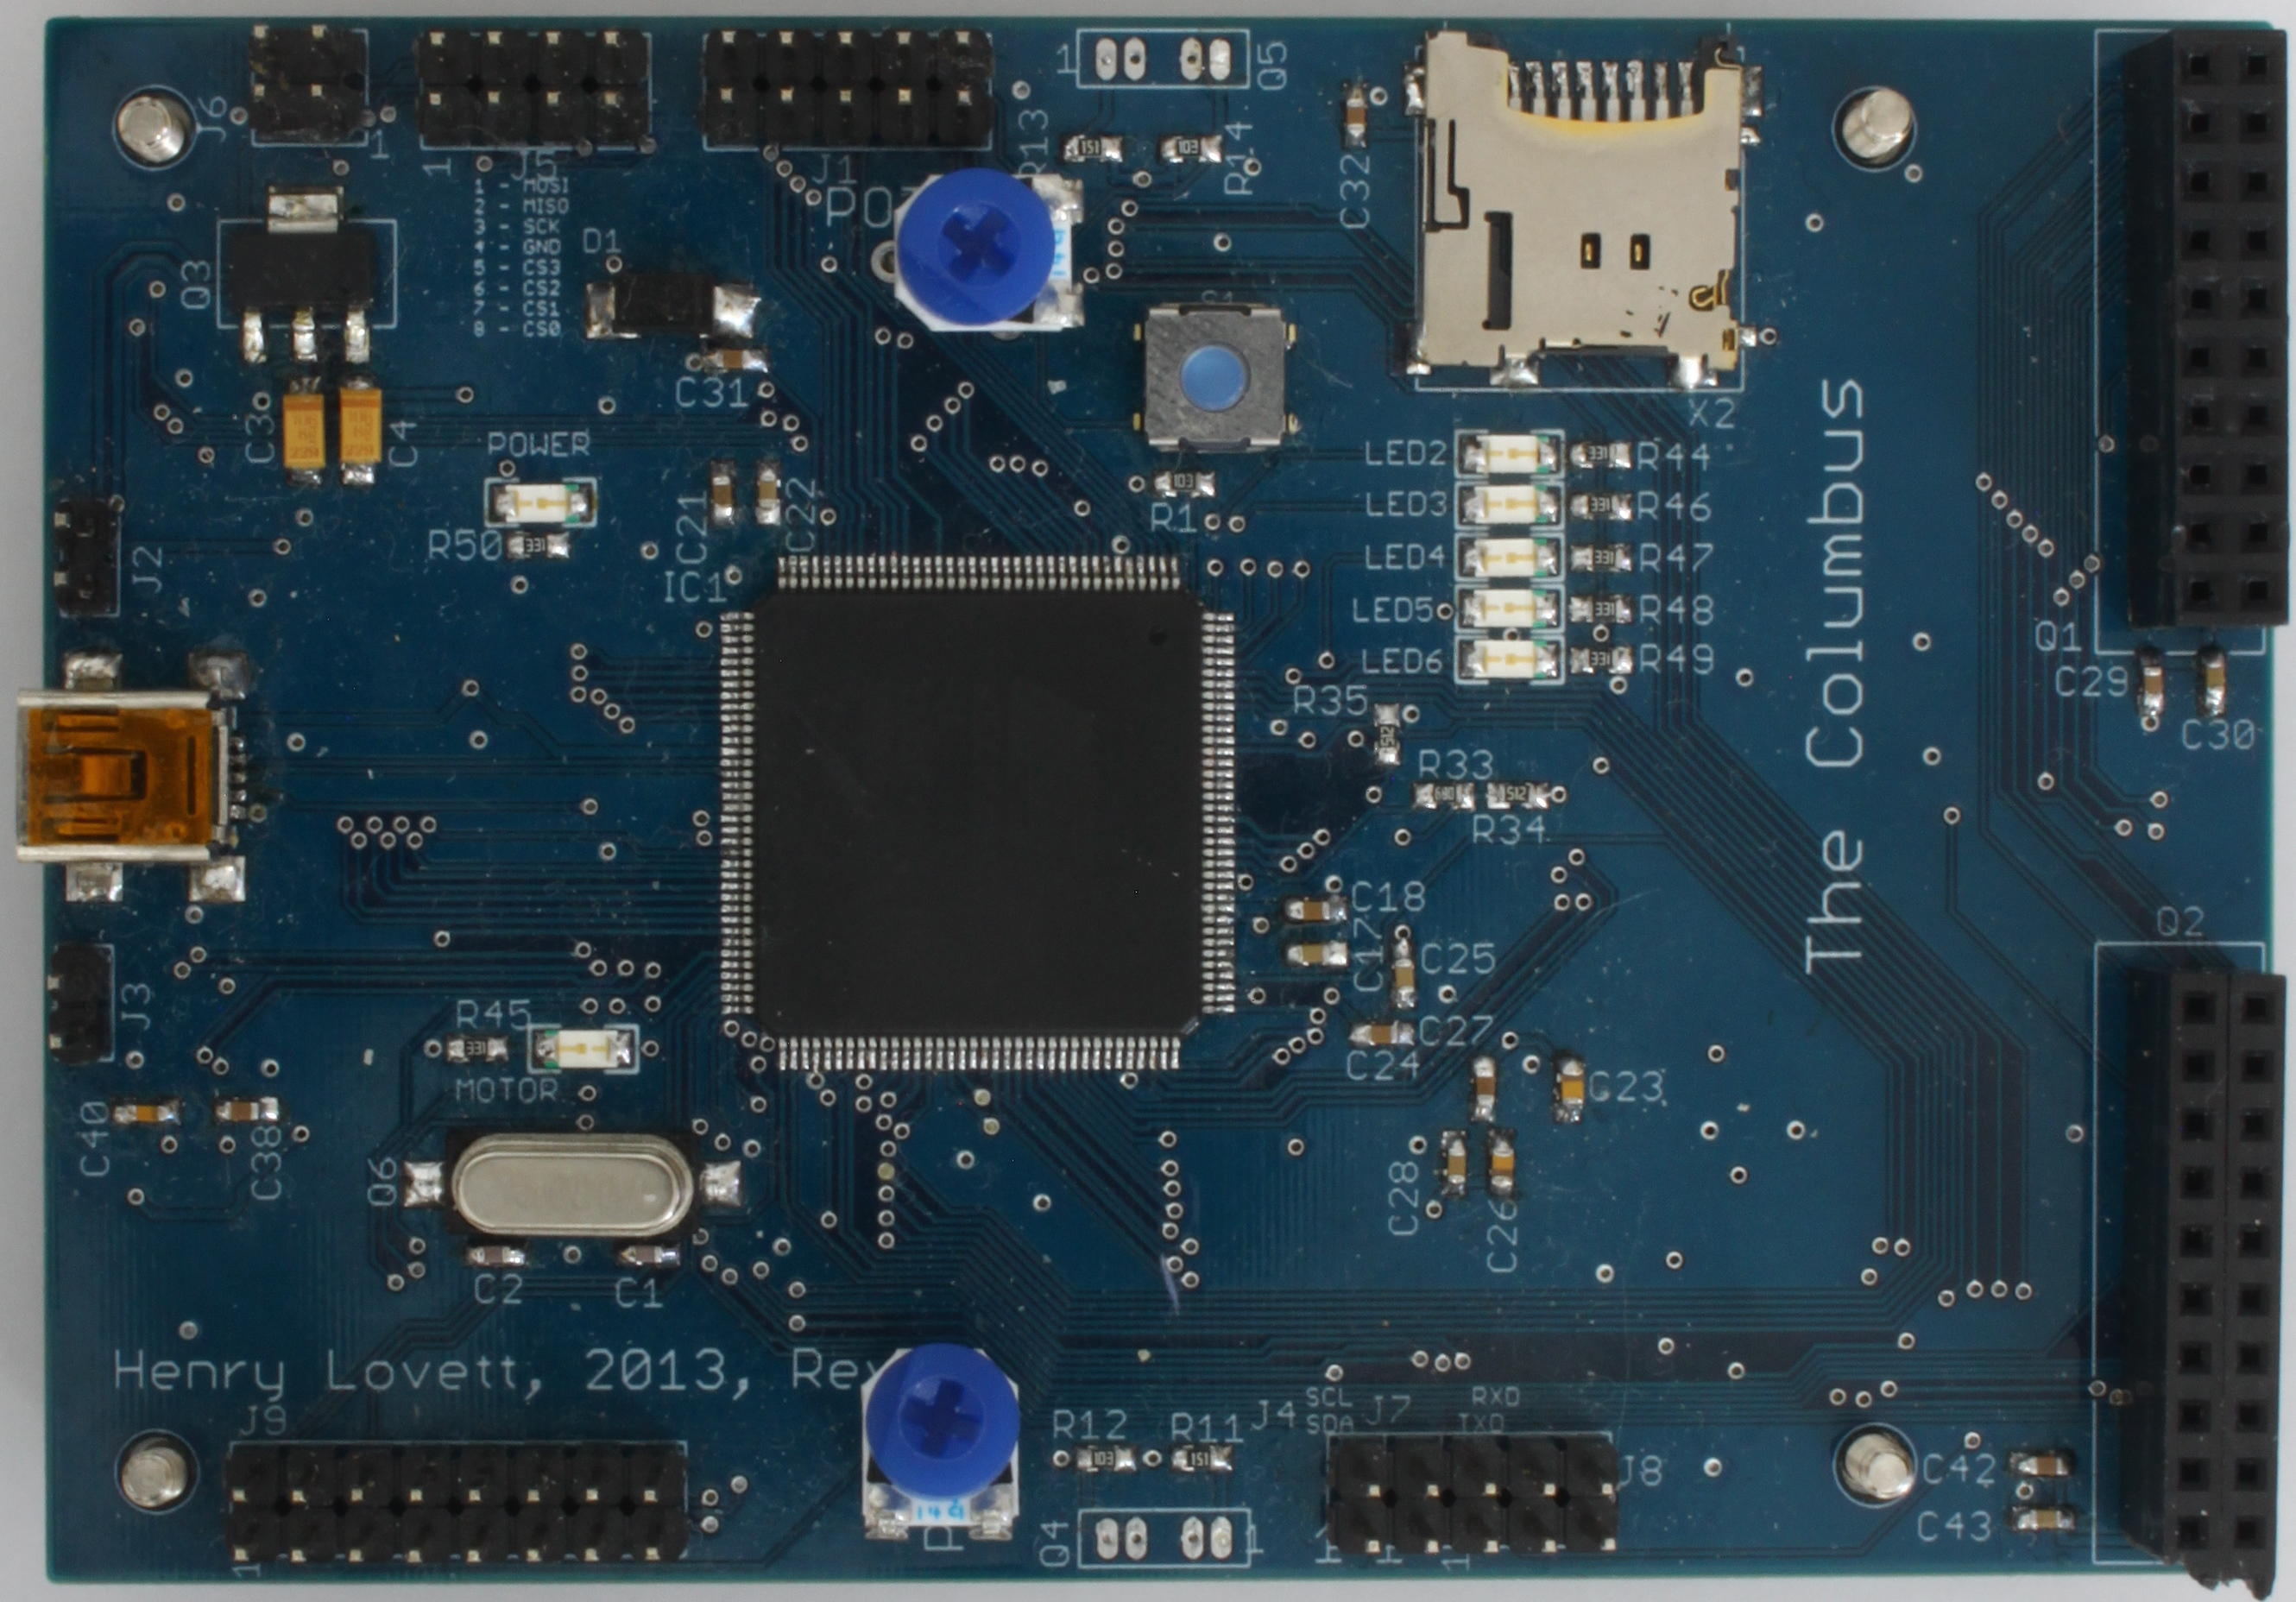
\includegraphics[width = \textwidth, keepaspectratio]{./Figures/PCB_Top.jpg} }
\subfigure[Bottom view of built PCB with SDRAM chip select patch \label{fig:PCB:Bottom}]{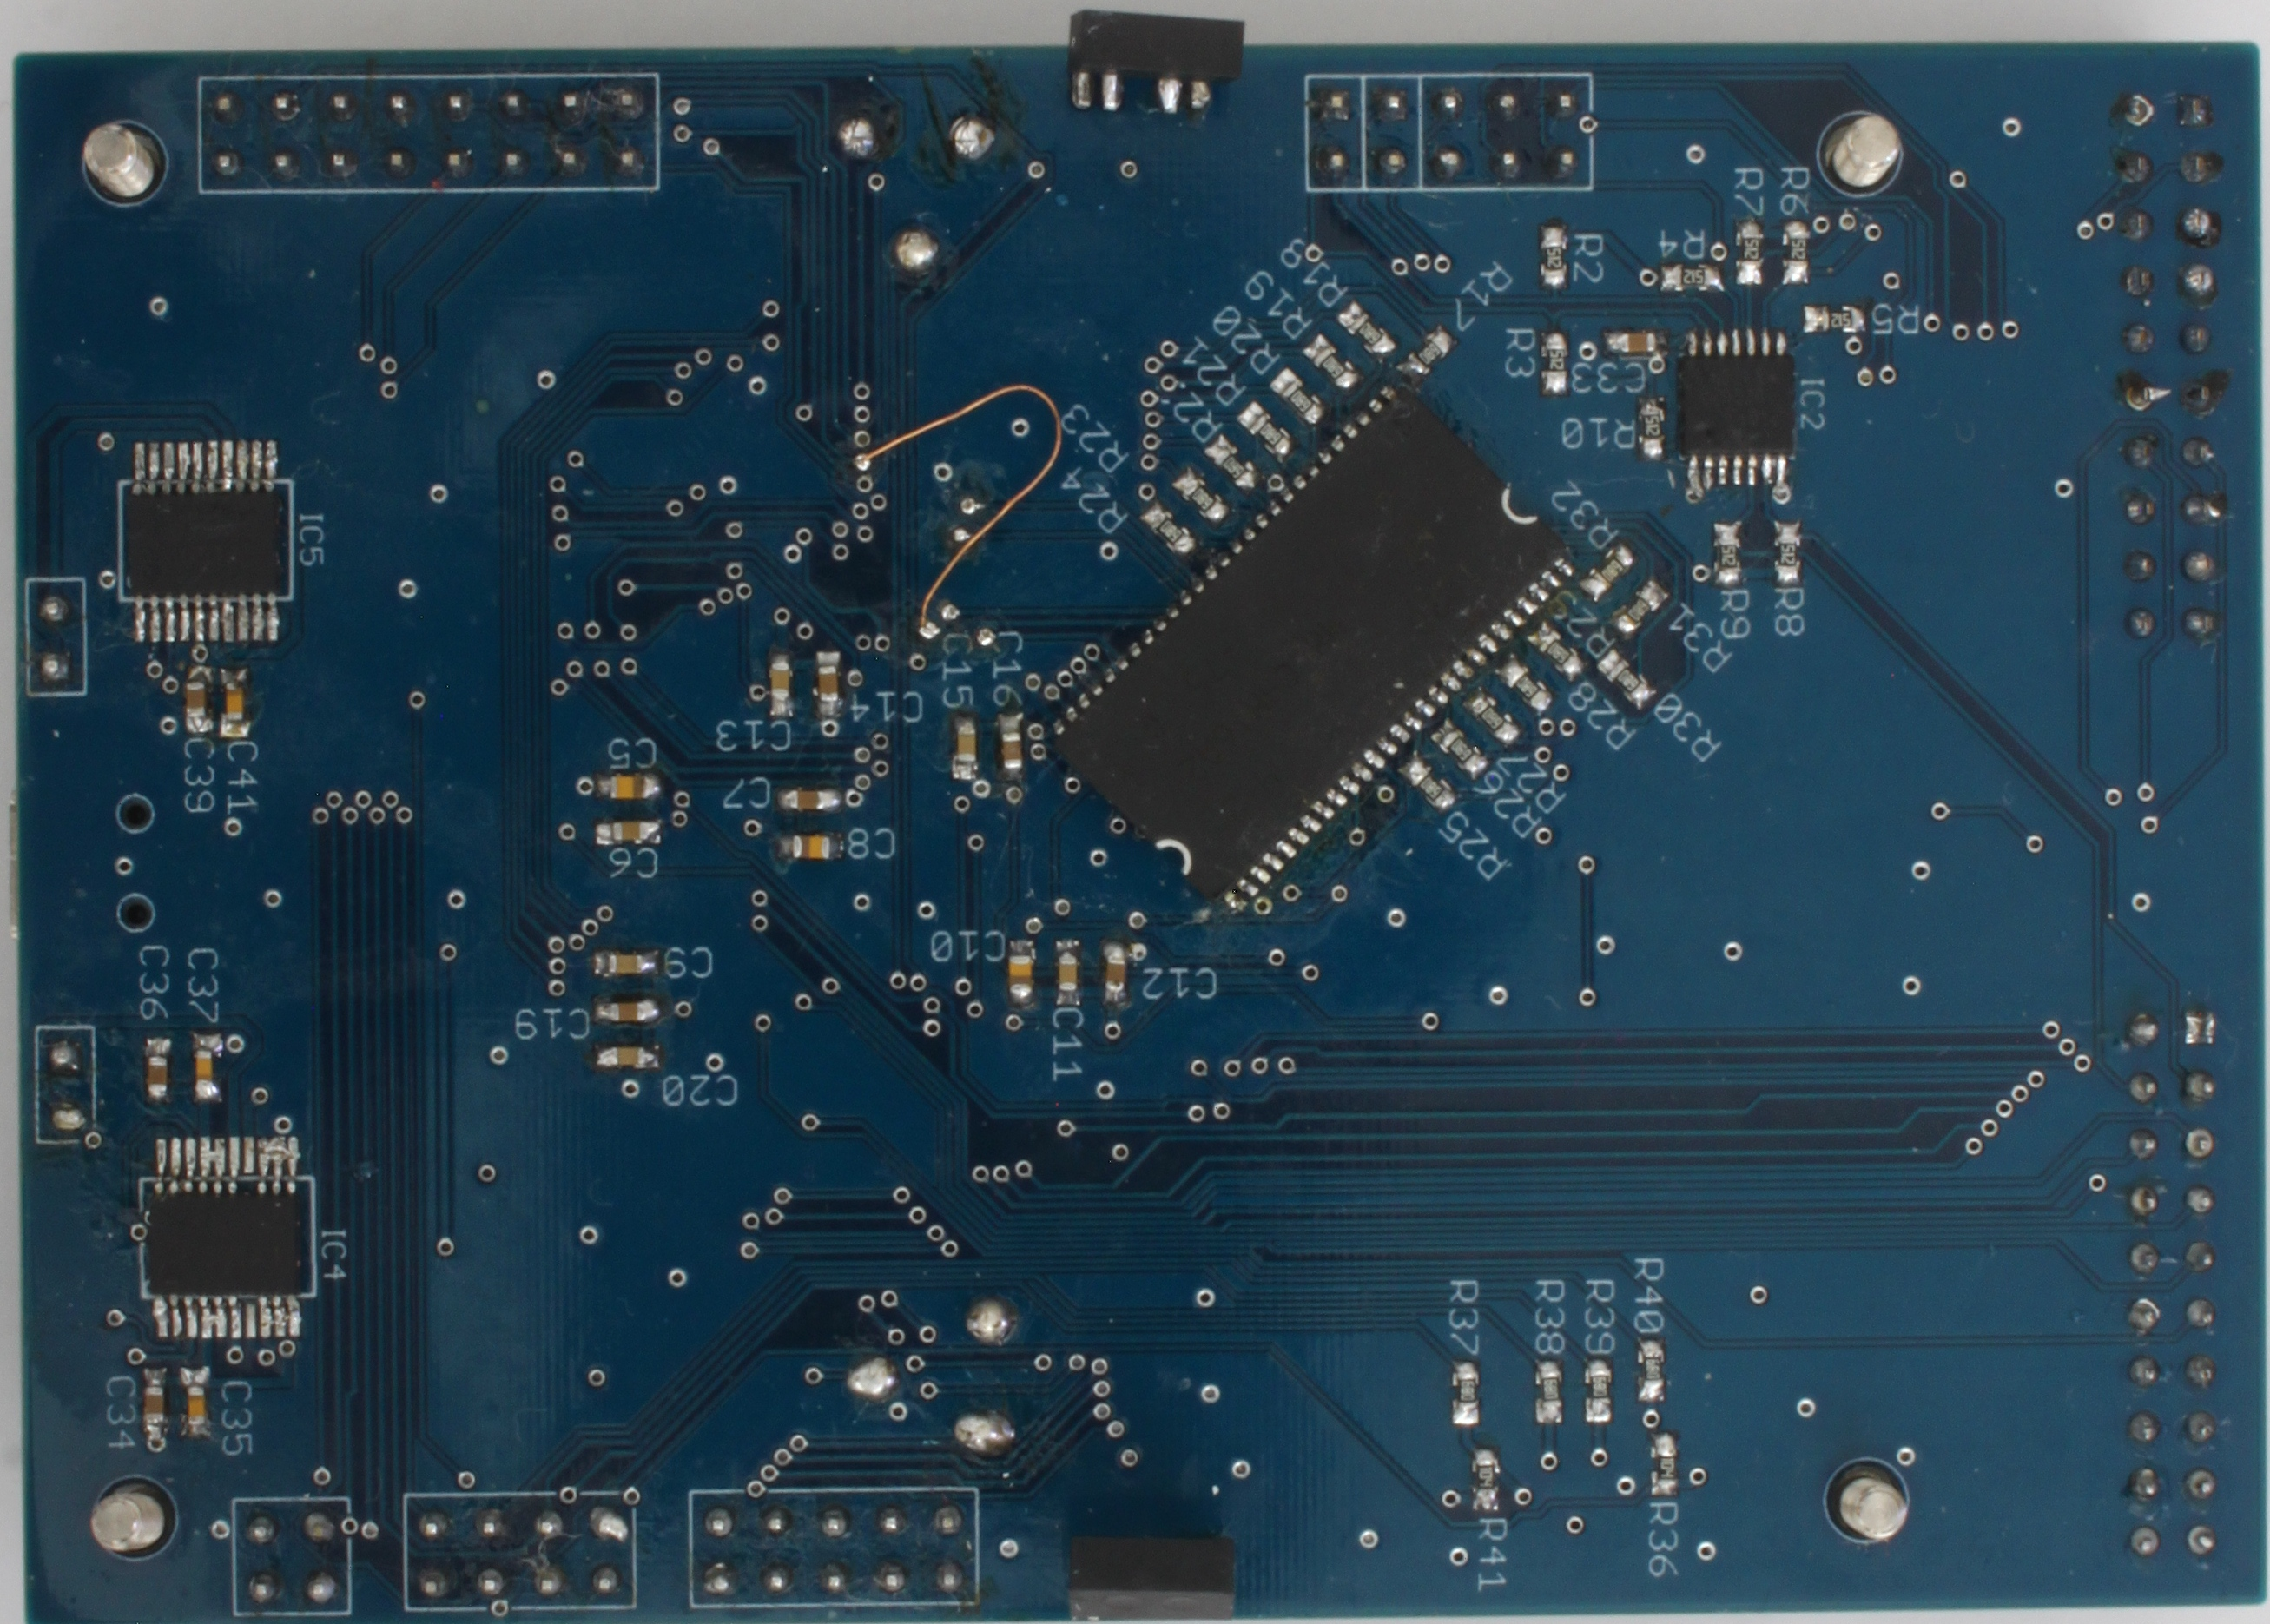
\includegraphics[width = \textwidth, keepaspectratio]{./Figures/PCB_Bottom.jpg} }
\caption{Pictures of the built PCB.}
\label{fig:PCB:Built}
\end{figure}
